\documentclass[crop=true, border=10pt]{standalone}
\usepackage{amsmath}
\usepackage{amsfonts}
\usepackage{mathrsfs}


\usepackage{graphicx} 
\usepackage{xcolor}

\usepackage{tikz}
\usetikzlibrary{arrows.meta}
\usetikzlibrary{decorations.markings}

\usepackage{tikz-3dplot}

\usepackage{pgfplots}


% A few colors 
%--------------------------------------------------------------
\definecolor{plum}{rgb}{0.36078, 0.20784, 0.4}
\definecolor{chameleon}{rgb}{0.30588, 0.60392, 0.023529}
\definecolor{cornflower}{rgb}{0.12549, 0.29020, 0.52941}
\definecolor{scarlet}{rgb}{0.8, 0, 0}
\definecolor{brick}{rgb}{0.64314, 0, 0}
\definecolor{sunrise}{rgb}{0.80784, 0.36078, 0}
\definecolor{lightblue}{rgb}{0.15,0.35,0.75}


%\pgfplotsset{width=7cm,compat=1.15}

\begin{document}


\pagestyle{empty}

%\begin{center}
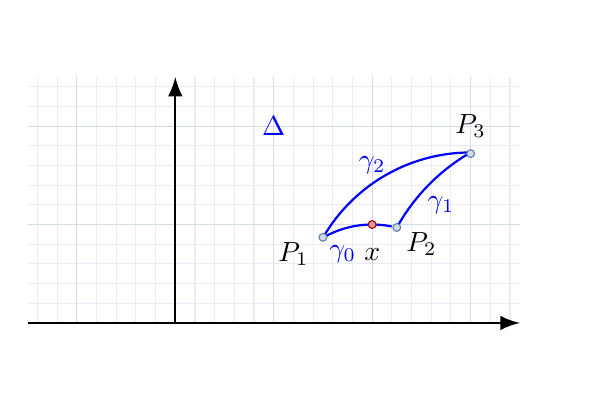
\begin{tikzpicture}[scale=1.25,domain=0:13]
	\tikzstyle{axisarrow} = [-{Latex[inset=0pt,length=7pt]}]

	% Clip all lines that would fall outside the grid
	\clip(-1.5,-0.5) rectangle (4,3);
	
	% Draw the grid.
	\draw [cornflower!10,step=0.2,thin] (-1.5,0) grid (3.5,2.5);
	\draw [cornflower!20,step=1.0,thin] (-1.5,0) grid (3.5,2.5);

	% \node[] at (6,-0.5) {Barn};
	% \node[] at (1.25,-0.5) {Pole};
	
	% Draw Axes
	\draw[thick,axisarrow] (0,0) -- (0,2.5);
	\draw[thick,axisarrow] (-1.5,0) -- (3.5,0);

	\draw [blue,thick,domain=1.5:2.2,samples=200] plot ({\x}, {sqrt(-(\x-2)^2 + 1 )});
    \draw [blue,thick,domain=2.26:3,samples=200] plot ({\x}, {sqrt(-(\x-4)^2 + 4 )});
    \draw [blue,thick,domain=1.5:3,samples=200] plot ({\x}, {sqrt(-(\x-3)^2 + 3 )});

    %Point
	\node at (2.25,0.97) [circle,draw=cornflower!70,fill=cornflower!20,inner sep=1pt] {};
    \node at (1.5,0.87) [circle,draw=cornflower!70,fill=cornflower!20,inner sep=1pt] {};
    \node at (3,1.72) [circle,draw=cornflower!70,fill=cornflower!20,inner sep=1pt] {};

    \node at (2,1) [circle,draw=brick,fill=brick!40,inner sep=1pt] {};

    %Letters
    \node at (1.2,0.7) [] {$P_1$};
	\node at (2.5,0.8) [] {$P_2$};
    \node at (3,2) [] {$P_3$};
    \node at (2,0.7) [] {$x$};
    \node[text = blue] at (1,2) [] {$\Delta$};

    \node[text = blue] at (1.7,0.7) [] {$\gamma_0$};
    \node[text = blue] at (2.7,1.2) [] {$\gamma_1$};
    \node[text = blue] at (2.0,1.6) [] {$\gamma_2$};
	
\end{tikzpicture}	
%\end{center}
			

\end{document}